\chapter{HIGGS BOSON MASS MEASUREMENT IN THE \texorpdfstring{\hzzfourl}{H to ZZ to 4l} CHANNEL}
\label{ch:higgs_mass}
% Need to use \texorpdfstring{} so it also shows in pdf bookmarks.
\section{Motivation}
When the CMS and ATLAS collaborations announced the discovery of the Higgs boson on July 4, 2012,
% TODO:cite
this was a momentous achievement in particle physics because the so-called ``missing'' piece of the SM was found.
Evidence of the Higgs boson's existence also motivates the associated Higgs field, which permeates all of spacetime and explains the origins of the masses of all the other massive fundamental particles (Chapter~\ref{ch:theory}).

The Higgs boson is interesting for a variety of reasons.
First, it is currently one of a kind---the only fundamental scalar particle ever discovered at the time of this writing.
Second, the mass of the Higgs boson theoretically determines the stability of our very Universe (Fig.~\ref{fig:universe_stability}).
Third, the unique boson could be a portal to new physics---\ie physics beyond the Standard Model (BSM)---\eg by decaying into BSM low-mass dilepton mass resonances (Chapter~\ref{ch:dilep_res}).
Fourth, the Higgs boson may not be the only one of its kind; some BSM models theorize that other kinds of Higgs bosons may exist.
% TODO:cite and double check.
Fifth, \emph{are we certain that the Higgs boson discovered in 2012 is the same as the one predicted by the SM?}
% In order to be certain that the recently discovered Higgs boson is truly the same as the one predicted by the SM, 
To check this, it is necessary to compare the Higgs boson's measured properties to its predicted ones.
One such property is the mass of the Higgs boson $\left( \mH \right)$.

This chapter details the measurement of \mH full Run 2 data from the LHC as analyzed by the CMS detector.
Although many previous measurements of \mH have already been made (\eg by the ATLAS and CMS collaborations as shown in Fig.~\ref{fig:atlas_cms_mH_meas}), the measurement presented in this dissertation gives the world's most precise value of \mH.
% ATLAS and CMS measurements of mH.
%%%%%%%%%%%%%%%%%%%%
\begin{figure}[hbtp]
    \centering
    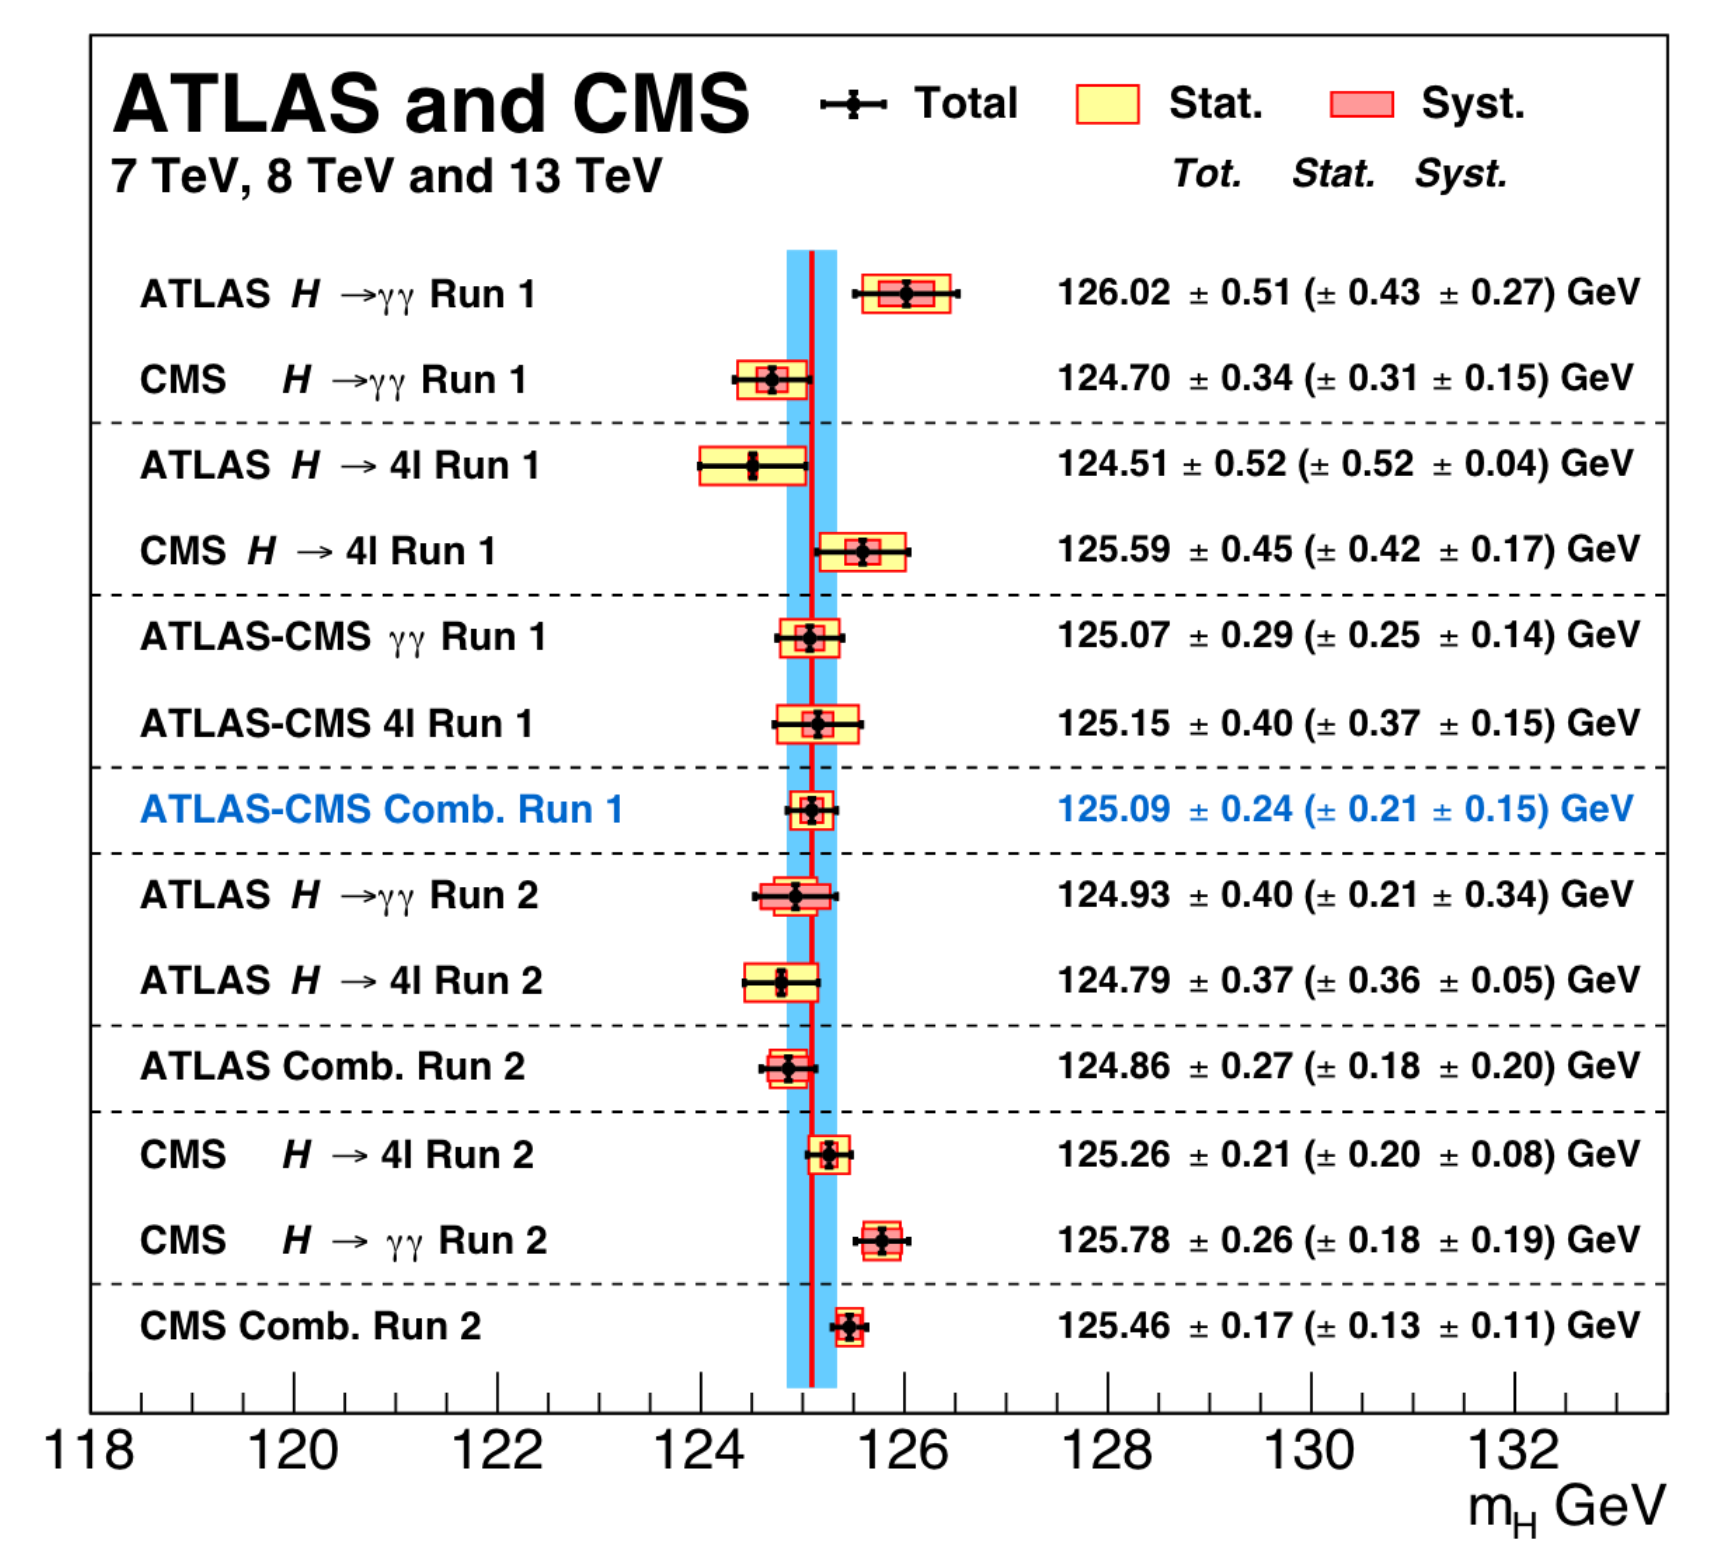
\includegraphics[width=\textwidth,keepaspectratio]{figures/higgsmassmeas/all_mH_measurements_atlas_cms.png}
        \caption
        [Various measurements of \mH made by the CMS and ATLAS collaborations.]
        {
            Various measurements of \mH made by the CMS and ATLAS collaborations in the \htoyy and \hzzfourl channels, in Runs 1 and 2 of the LHC.
            Plot taken from~\cite{particle_data_group_review_2020}.
        }
        \label{fig:atlas_cms_mH_meas}
\end{figure}
%%%%%%%%%%%%%%%%%%%%
% Some properties of the Higgs boson can be predicted by the SM, like 
%     - There are many results on Higgs properties: spin, charge, decay processes, lifetime, mass.
%     - The last of these is the focus of this dissertation and is of particular importance to the Universe: depending on mH and mtop, the stability of the Universe.

% - Why this thesis is important:
%     - This thesis describes the methodology and results of the best precision measurement of mH to date by using the hZZ4l decay and Full Run 2 data set from CMS.
%     - Run 2 provides more data -> more precision on measurements of Higgs properties.
%     - In addition to more HZZ4l events, this analysis provides new techniques, specifically the VX constraint.
%     - Predict mH for Run 3, will start soon summer 2022 and provide an approximate 300? /fb of L int.
%     - In 2026(?), HLLHC provides even more data. ref snowmass paper.

First, a general overview of the logic and analysis workflow for the \mH measurement is motivated in Sec.~\ref{sec:analysis_overview}.
The specific data sets, simulated samples, and triggers used in the analysis are then detailed in Sec.~\ref{sec:analyzed_data}.
Then the event reconstruction and event selection are described in Sec.~\ref{sec:evt_sel}.
Afterwards, an analysis of the background estimation is given in Sec.~\ref{sec:bkg_estim}.
The signal modeling and improvements utilized in this measurement are then laid out, which include the kinematic discriminant, per-event mass uncertainties, and the vertex constraint in Sec.~\ref{sec:signal_model}.
A treatment of the systematic uncertainties follows in Sec.~\ref{sec:syst_uncert}.
The chapter concludes with a summary of the \mH measurement results in Sec.~\ref{sec:results}.

% \begin{itemize}                                                                          
%     \item Sec.~\ref{sec:analysis_overview}: General overview of the analysis of the Higgs boson mass measurement.
%     \item Sec.~\ref{sec:analyzed_data}: Data sets, triggers, and simulation.
%     \item Sec.~\ref{sec:evt_sel}: Event reconstruction and selection.
%     \item Sec.~\ref{sec:bkg_estim}: Background estimation.
%     \item Sec.~\ref{sec:signal_model}: Signal modeling and improvements, including kinematic discriminant, per-event mass uncertainties, VXBS constraint, reference to ad hoc studies in appendix.
%     % \item Observables: Four-Lepton Invariant Mass, Per-Event Mass Uncertainty, Matrix Element-Based Kinematic Discriminant) (Sec.~\ref{sec:observables})
%     \item Sec.~\ref{sec:syst_uncert}: Systematic uncertainties.
%     \item Sec.~\ref{sec:results}: Results.
% \end{itemize}
